\documentclass[tikz]{standalone}
\usetikzlibrary{patterns}
\usetikzlibrary{shapes,arrows.meta}
\usetikzlibrary{decorations.pathreplacing, positioning}
\definecolor{greengreen}{rgb}{0.0, 0.42, 0.24}
\definecolor{calpolypomonagreen}{rgb}{0.12, 0.3, 0.17}
\definecolor{forestgreen}{rgb}{0.13, 0.55, 0.13}

\begin{document}
\noindent
  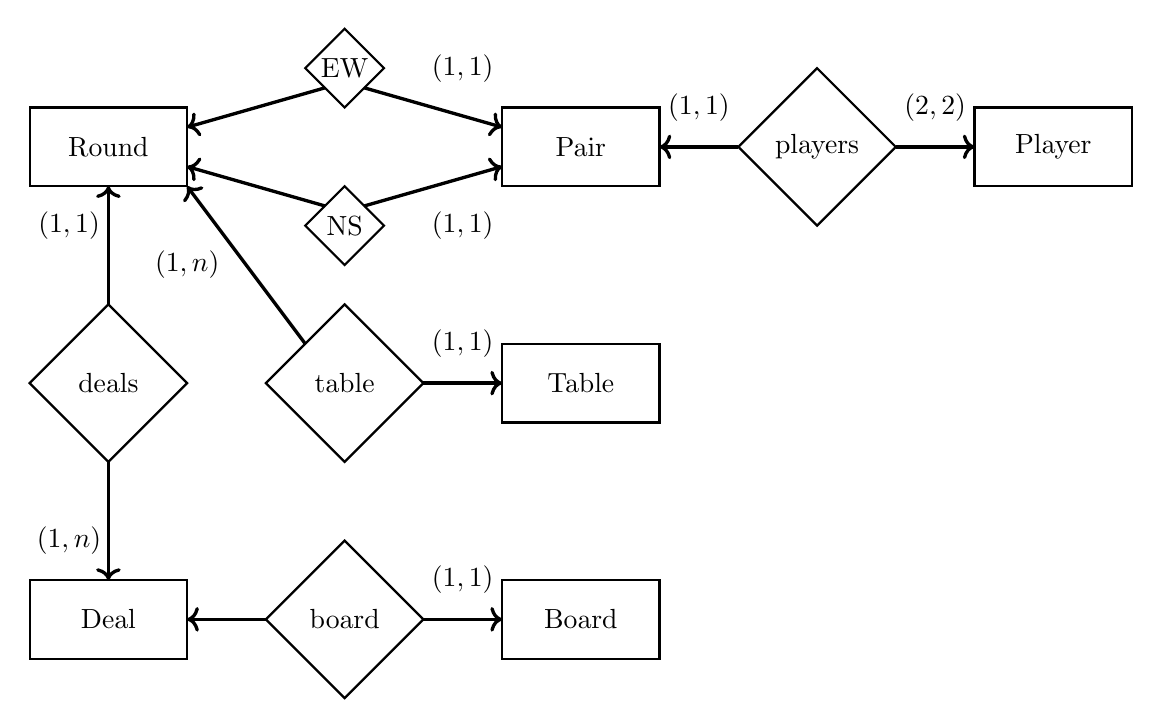
\begin{tikzpicture}

    % Round
    \draw[thick] (0,0) rectangle (2,1);
    \node[align=center] at (1,0.5) {Round};

    % Pair
    \draw[thick] (6,0) rectangle (8,1);
    \node[align=center] at (7,0.5) {Pair};

    % Player
    \draw[thick] (12,0) rectangle (14,1);
    \node[align=center] at (13,0.5) {Player};
    
    % Table
    \draw[thick] (6,-3) rectangle (8,-2);
    \node[align=center] at (7, -2.5) {Table};

    % Deal
    \draw[thick] (0,-6) rectangle (2,-5);
    \node[align=center] at (1,-5.5) {Deal};

    % Board
    \draw[thick] (6,-6) rectangle (8,-5);
    \node[align=center] at (7,-5.5) {Board};

    % ================================
    % Diamonds

    % deals
    \draw[thick] (0,-2.5) -- (1,-1.5) -- (2,-2.5) -- (1,-3.5) -- cycle;
    \node[align=center] at (1,-2.5) {deals};
    \draw[very thick, ->] (1, -1.5) -- (1,0);
    \draw[very thick, ->] (1, -3.5) -- (1,-5);

    % board
    \draw[thick] (3, -5.5) -- (4,-4.5) -- (5,-5.5) -- (4,-6.5) -- cycle;
    \node[align=center] at (4,-5.5) {board};
    \draw[very thick, ->] (3, -5.5) -- (2, -5.5);
    \draw[very thick, ->] (5, -5.5) -- (6, -5.5);

    % table
    \draw[thick] (3, -2.5) -- (4,-1.5) -- (5,-2.5) -- (4,-3.5) -- cycle;
    \node[align=center] at (4,-2.5) {table};
    \draw[very thick, ->] (3.5, -2) -- (2, 0);
    \draw[very thick, ->] (5, -2.5) -- (6, -2.5);

    % NS
    \draw[thick] (3.5, -0.5) -- (4,-0) -- (4.5,-0.5) -- (4,-1) -- cycle;
    \node[align=center] at (4,-0.5) {NS};
    \draw[very thick, ->] (3.75, -0.25) -- (2, 0.25);
    \draw[very thick, ->] (4.25, -0.25) -- (6, 0.25);

    % EW
    \draw[thick] (3.5, 1.5) -- (4,2) -- (4.5,1.5) -- (4,1) -- cycle;
    \node[align=center] at (4,1.5) {EW};
    \draw[very thick, ->] (3.75, 1.25) -- (2, 0.75);
    \draw[very thick, ->] (4.25, 1.25) -- (6, 0.75);

    % players
    \draw[thick] (9, 0.5) -- (10,1.5) -- (11,0.5) -- (10,-0.5) -- cycle;
    \node[align=center] at (10,0.5) {players};
    \draw[very thick, ->] (9, 0.5) -- (8, 0.5);
    \draw[very thick, ->] (11, 0.5) -- (12, 0.5);

    % ================================
    % Values

    \node[align=center] at (5.5, -0.5) {$(1,1)$};
    \node[align=center] at (5.5, 1.5) {$(1,1)$};

    \node[align=center] at (8.5, 1) {$(1,1)$};
    \node[align=center] at (11.5, 1) {$(2,2)$};
    
    \node[align=center] at (0.5, -0.5) {$(1,1)$};
    \node[align=center] at (0.5, -4.5) {$(1,n)$};

    \node[align=center] at (2, -1) {$(1,n)$};
    \node[align=center] at (5.5, -2) {$(1,1)$};

    \node[align=center] at (5.5, -5) {$(1,1)$};

  \end{tikzpicture}%
\end{document}
